\begin{figure}
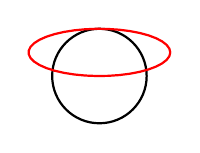
\begin{tikzpicture}[scale=.6]
	\drawgrid{-2.5}{-2.5}{2.5}{2.5}
	\draw[thick] (0, 0) circle [radius=1];
	\draw[thick, red] plot[domain=0:360, samples=40]
		({cos(\x)*1.5},{0.5+sin(\x)*0.5});
	\draw[thick, blue] plot[domain=-1.301:4.444,
		samples=150] ({\inverseellipseX},
		{\inverseellipseY});
\end{tikzpicture}
	\caption{ $E(x, y, z)$ }
	\label<5>{fig:ellipse5}
\end{figure}
